\documentclass[tikz,border=5pt]{standalone}
\usepackage{tikz}

\begin{document}
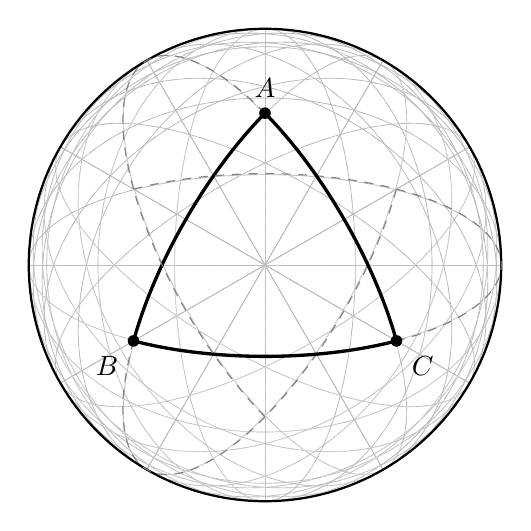
\begin{tikzpicture}[scale=3, line cap=round, line join=round]

  % Styles
  \tikzset{
    gridFront/.style={line width=0.25pt, gray!55},
    gridBack/.style={line width=0.25pt, gray!35, dashed},
    tri/.style={very thick}
  }

  % --- Geodesic grid (great circles) behind ---
  \begin{scope}
    \clip (0,0) circle (1);

    % Helper: draw a full great circle from its plane normal n=(nx,ny,nz)
    % Front (z>=0) solid, back (z<0) dashed.
    \newcommand{\DrawGreatCircle}[3]{%
      \pgfmathsetmacro{\nx}{#1}\pgfmathsetmacro{\ny}{#2}\pgfmathsetmacro{\nz}{#3}
      \pgfmathsetmacro{\plen}{sqrt(\nx*\nx + \ny*\ny)}
      \ifdim \plen pt < 0.000001pt
        % n parallel to z (equator) -> skip to avoid overdrawing the rim
      \else
        % Orthonormal basis for the circle in 3D (projected to xy)
        \pgfmathsetmacro{\ux}{-\ny/\plen}
        \pgfmathsetmacro{\uy}{ \nx/\plen}
        \pgfmathsetmacro{\uz}{ 0}
        \pgfmathsetmacro{\vx}{-\nz*\nx/\plen}
        \pgfmathsetmacro{\vy}{-\nz*\ny/\plen}
        \pgfmathsetmacro{\vz}{ \plen}
        % Back half: t in [-180,0], Front half: t in [0,180] since z(t)=vz*sin(t)
        \draw[gridBack]
          plot[domain=-180:0, samples=140, variable=\t]
            ({\ux*cos(\t)+\vx*sin(\t)}, {\uy*cos(\t)+\vy*sin(\t)});
        \draw[gridFront]
          plot[domain=0:180, samples=140, variable=\t]
            ({\ux*cos(\t)+\vx*sin(\t)}, {\uy*cos(\t)+\vy*sin(\t)});
      \fi
    }

    % 1) Meridians (planes through the viewing axis): every 30�
    \foreach \phi in {0,30,...,330}{
      \pgfmathsetmacro{\nx}{cos(\phi)}
      \pgfmathsetmacro{\ny}{sin(\phi)}
      \pgfmathsetmacro{\nz}{0}
      \DrawGreatCircle{\nx}{\ny}{\nz}
    }

    % 2) Tilted families (normals at fixed tilt from the pole), rotated every 30�
    \foreach \tilt in {22.5,45,67.5}{
      \foreach \phi in {0,30,...,330}{
        \pgfmathsetmacro{\nx}{sin(\tilt)*cos(\phi)}
        \pgfmathsetmacro{\ny}{sin(\tilt)*sin(\phi)}
        \pgfmathsetmacro{\nz}{cos(\tilt)}
        \DrawGreatCircle{\nx}{\ny}{\nz}
      }
    }
  \end{scope}

  % Sphere outline on top
  \draw[thick] (0,0) circle (1);

  % --- Symmetric triangle on the front hemisphere ---
  % All three vertices share the same latitude; longitudes 120� apart
  \pgfmathsetmacro{\lat}{50} % >0 to lie on the front hemisphere
  \pgfmathsetmacro{\lonA}{ 90}
  \pgfmathsetmacro{\lonB}{210}
  \pgfmathsetmacro{\lonC}{330}

  % Convert to 3D unit vectors (degrees; x=cosf cos?, y=cosf sin?, z=sinf)
  \pgfmathsetmacro{\Ax}{cos(\lat)*cos(\lonA)}
  \pgfmathsetmacro{\Ay}{cos(\lat)*sin(\lonA)}
  \pgfmathsetmacro{\Az}{sin(\lat)}

  \pgfmathsetmacro{\Bx}{cos(\lat)*cos(\lonB)}
  \pgfmathsetmacro{\By}{cos(\lat)*sin(\lonB)}
  \pgfmathsetmacro{\Bz}{sin(\lat)}

  \pgfmathsetmacro{\Cx}{cos(\lat)*cos(\lonC)}
  \pgfmathsetmacro{\Cy}{cos(\lat)*sin(\lonC)}
  \pgfmathsetmacro{\Cz}{sin(\lat)}

  % Helper: draw the short great-circle arc from P to Q (opposite half dashed)
  \newcommand{\DrawGCArc}[9]{%
    \pgfmathsetmacro{\nx}{#1}\pgfmathsetmacro{\ny}{#2}\pgfmathsetmacro{\nz}{#3}
    \pgfmathsetmacro{\px}{#4}\pgfmathsetmacro{\py}{#5}\pgfmathsetmacro{\pz}{#6}
    \pgfmathsetmacro{\qx}{#7}\pgfmathsetmacro{\qy}{#8}\pgfmathsetmacro{\qz}{#9}
    \pgfmathsetmacro{\plen}{sqrt(\nx*\nx + \ny*\ny)}
    \pgfmathsetmacro{\ux}{-\ny/\plen}
    \pgfmathsetmacro{\uy}{ \nx/\plen}
    \pgfmathsetmacro{\uz}{ 0}
    \pgfmathsetmacro{\vx}{-\nz*\nx/\plen}
    \pgfmathsetmacro{\vy}{-\nz*\ny/\plen}
    \pgfmathsetmacro{\vz}{ \plen}
    \pgfmathsetmacro{\cuP}{\px*\ux + \py*\uy + \pz*\uz}
    \pgfmathsetmacro{\cvP}{\px*\vx + \py*\vy + \pz*\vz}
    \pgfmathsetmacro{\tP}{atan2(\cvP,\cuP)}
    \pgfmathsetmacro{\cuQ}{\qx*\ux + \qy*\uy + \qz*\uz}
    \pgfmathsetmacro{\cvQ}{\qx*\vx + \qy*\vy + \qz*\vz}
    \pgfmathsetmacro{\tQ}{atan2(\cvQ,\cuQ)}
    \pgfmathsetmacro{\dAng}{mod(\tQ-\tP+540,360)-180}
    \draw[tri]
      plot[domain=\tP:\tP+\dAng, samples=160, variable=\t]
        ({\ux*cos(\t)+\vx*sin(\t)}, {\uy*cos(\t)+\vy*sin(\t)});
    \draw[gray, dashed]
      plot[domain=\tP+\dAng:\tP+\dAng+180, samples=140, variable=\t]
        ({\ux*cos(\t)+\vx*sin(\t)}, {\uy*cos(\t)+\vy*sin(\t)});
  }

  % Great-circle normals for triangle edges: n = P x Q (unitized)
  % AB
  \pgfmathsetmacro{\nABx}{\Ay*\Bz - \Az*\By}
  \pgfmathsetmacro{\nABy}{\Az*\Bx - \Ax*\Bz}
  \pgfmathsetmacro{\nABz}{\Ax*\By - \Ay*\Bx}
  \pgfmathsetmacro{\nABn}{sqrt(\nABx*\nABx + \nABy*\nABy + \nABz*\nABz)}
  \pgfmathsetmacro{\nABx}{\nABx/\nABn}
  \pgfmathsetmacro{\nABy}{\nABy/\nABn}
  \pgfmathsetmacro{\nABz}{\nABz/\nABn}
  % BC
  \pgfmathsetmacro{\nBCx}{\By*\Cz - \Bz*\Cy}
  \pgfmathsetmacro{\nBCy}{\Bz*\Cx - \Bx*\Cz}
  \pgfmathsetmacro{\nBCz}{\Bx*\Cy - \By*\Cx}
  \pgfmathsetmacro{\nBCn}{sqrt(\nBCx*\nBCx + \nBCy*\nBCy + \nBCz*\nBCz)}
  \pgfmathsetmacro{\nBCx}{\nBCx/\nBCn}
  \pgfmathsetmacro{\nBCy}{\nBCy/\nBCn}
  \pgfmathsetmacro{\nBCz}{\nBCz/\nBCn}
  % CA
  \pgfmathsetmacro{\nCAx}{\Cy*\Az - \Cz*\Ay}
  \pgfmathsetmacro{\nCAy}{\Cz*\Ax - \Cx*\Az}
  \pgfmathsetmacro{\nCAz}{\Cx*\Ay - \Cy*\Ax}
  \pgfmathsetmacro{\nCAn}{sqrt(\nCAx*\nCAx + \nCAy*\nCAy + \nCAz*\nCAz)}
  \pgfmathsetmacro{\nCAx}{\nCAx/\nCAn}
  \pgfmathsetmacro{\nCAy}{\nCAy/\nCAn}
  \pgfmathsetmacro{\nCAz}{\nCAz/\nCAn}

  % Draw triangle edges (short great-circle arcs)
  \DrawGCArc{\nABx}{\nABy}{\nABz}{\Ax}{\Ay}{\Az}{\Bx}{\By}{\Bz}
  \DrawGCArc{\nBCx}{\nBCy}{\nBCz}{\Bx}{\By}{\Bz}{\Cx}{\Cy}{\Cz}
  \DrawGCArc{\nCAx}{\nCAy}{\nCAz}{\Cx}{\Cy}{\Cz}{\Ax}{\Ay}{\Az}

  % Vertex markers and labels (projected positions)
  \fill (\Ax,\Ay) circle (0.7pt) node[above=2pt] {$A$};
  \fill (\Bx,\By) circle (0.7pt) node[below left=2pt] {$B$};
  \fill (\Cx,\Cy) circle (0.7pt) node[below right=2pt] {$C$};

\end{tikzpicture}
\end{document}
